\section{Example: The Linear System Analyzer}
\label{sec:lsa}

% 
% IV. Example: LSA
% 
%     A. Application domain covered, components, example workflow
% 
%     B. SWIM files (c.f. III.B.2) for reorder, splib
% 
%     C. Component scripts for reorder, splib
% 
%     D. Overall script for an example workflow
% 
%     E. Screen shots: customize, event log, event query, script uploaded,
%         splib-generated web page.
% 
% V. Example: AORSA + CQL
% 

As a brief example of how an application can be assembled and run in the
SWIM framework, a set of serial codes have been wrapped up as separate
executables. The codes are a subset drawn from the Linear System Analyzer
(LSA) \cite{lsa_book},  an early component-based problem-solving environment for
developing solution strategies for sparse linear systems of equations. The
modules that have been adapted are in Table \ref{lsacomponents}.
Each reads in a sparse linear
system's coefficient matrix and right hand side vector in "coordinate-wise"
format from a file called {\em mat.in}.  Most also take an input parameter file
called {\em methods}. Three general categories of LSA components have been
identified based on their dataflows.
A {\bf filter} component modifies the linear system and produces
another one in mat.out.  An {\bf informational} component gives data such as the
number of nonzeros, a measure of symmetry, etc. A {\bf solver} (tries to) solve
the linear system, and also produces some information garnered about the linear
system during the solve - the main purpose of the LSA.

\begin{table}
    \begin{center}
        \begin{tabular}{||l|l|l|l||} \hline \hline
            {\bf Name}      &  {\bf Type}      & {\bf Inputs}     & {\bf Outputs} \\ \hline \hline
			BasicInfo       &  Informational   &  mat.in          &  mat.html + GIF \\ 
			                &                  &                  &  files        \\ \hline
			Scale           &  Filter          &  mat.in, methods &  mat.out,     \\
			                &                  &                  &  summary.html \\ \hline
			Reorder         &  Filter          &  mat.in, methods &  mat.out      \\ \hline
			Splib           &  Solver          &  mat.in, methods &  results.html,\\
			                &                  &                  &  PNG files    \\ \hline
			SuperLU         &  Solver          &  mat.in, methods &  info.html    \\ \hline \hline
        \end{tabular}
    \end{center}
    \caption{\label{lsacomponents} Sample LSA Components}
\end{table}

Several other solvers and filters are possible and were in the original
LSA, but these are sufficient to put together simple workflows. An example
is in Figure \ref{lsaworkflow}, where the moving of one component's output file to
another's input file is shown by an arrow. That example workflow would allow a user
to compare the effects of scaling and not scaling the coefficient matrix,
for both an interative (Splib) and sparse direct (SuperLU) solver.
\begin{figure}
\centering
% \includegraphics[height=3.1in]{arch}
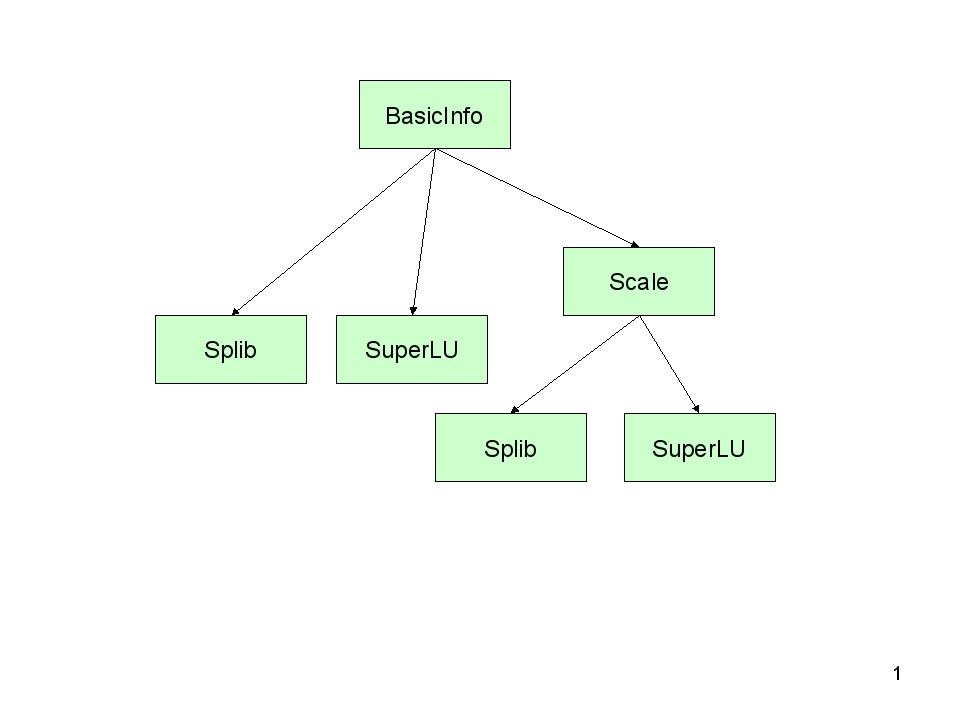
\includegraphics[width=4.0in]{tree}
\caption{Example LSA workflow}
\label{lsaworkflow}
\end{figure}

The LSA is not a high-performance system and all of the codes are serial.
The intent is to allow comparison of algorithms and preconditioning, not
for scalable parallelism. It has proven useful as a guide in choosing a HPC
solution strategy (filtering, preconditioning, solver method) but does not
supply or replace one.

The LSA provides a simple example of scripting an application using Python
and for using framework services.
